\section{\name Design}\label{sec:design}\label{s:design}
\name is a \emph{reconfigurable} and \emph{extensible} network stack. We start by defining these terms.

\paragrapha{Reconfigurability} refers to an application's ability to choose between different implementations of the same functionality both \emph{when} establishing a connection and \emph{after} the connection has been established. In practice, this means \name allows applications to choose among \tunnels that implement similar functionality, \eg between DPDK and kernel networking in Figure~\ref{f:chunnel-basic}. As we discussed earlier, choosing \tunnels (\ie reconfiguration) when establishing connections allows applications to be specialized to where they are deployed. Similarly, reconfiguration after a connection has been established is useful when \tunnel performance and efficiency vary depending on workload characteristics or resource availability, since it allows the application to respond to changes without disrupting ongoing connections. For example, DPDK \tunnels can be built either so they poll for I/O in the application thread---which requires pinning the application thread to a dedicated core but provides low latency---or to use a shared I/O core for polling---which makes it easier to share cores between applications but increases latency due to IPC. The choice between these two alternatives depends on the number of cores that are available and on the observed workload. \name's runtime reconfiguration process allows administrators (or orchestrators) to change how I/O is performed at runtime without disrupting existing connections.



\paragrapha{Extensible} refers to the application and library developer's ability to add new \tunnels to \name. These \tunnels can either represent alternate implementations of the same functionality or entirely new functions. Extensibility allows \name's reconfiguration to allow changes not just to the lowest layers of the network stack, but also to allow changes to how more complex communication primitives are implemented.

Supporting both reconfigurability and extensibility imposes four design requirements on \name:
\begin{compactenum}
\item Switching between two \tunnels that implement the same functionality should not require changes to application logic.
\item Reconfiguration should be \emph{safe}; it should not lead to scenarios where a connected host can no longer communicate. Some \tunnels, \eg serialization \tunnels, require all communicating hosts to use compatible formats, and \name must ensure that this holds.
\item Reconfigurability should neither limit what \tunnels an application can compose nor limit what functionality a \tunnel can implement.%
\item When possible, reconfiguring an established connection should not require re-establishing the connection state.
\end{compactenum}

The \tunnel abstraction meets most of these requirements by enforcing a unified interface that ensures that \tunnels can be composed and reconfigured. However, the abstraction alone is insufficient for ensuring safety, and the \name runtime implements a negotiation protocol (\S\ref{s:negotiation}) that checks compatibility between hosts when establishing or re-configuring connections.
For reference, we provide in Table~\ref{t:glossary} a glossary of \name's important concepts.
\begin{table}[t]
    \centering
    \small
    \begin{tabular}{p{1.7cm} p{5.7cm}}
        \tunnel & A specific piece of network functionality. \\
        \hline
        \tunnel stack & An application's specification of the set of \tunnels it wants to use. \\
        \hline
        Reconfiguration & Picking or changing \tunnel implementations for a connection at runtime. \\
        \hline
        Negotiation & Ensuring that \tunnel implementations are compatible across connection endpoints. \\
    \end{tabular}
    \vspace{10pt}
    \caption{Glossary of terms used in this paper.}
    \label{t:glossary}
\end{table}






\begin{listing}[t!]
\begin{minted}[linenos, breaklines]{rust}
// Client-side application code.
let sock = KernelUdpChunnel::new(); // () -> bytes
let shrd = ClientShard::new(cfg); // T -> T + sharding
let ser = SerializeChunnel::new(idl); // bytes -> type T
let conn = tbm::make_stack!(ser, shrd, sock).connect(addr);
\end{minted}
\vspace{-12pt}
\caption{An application developer specifies a \tunnel stack (\texttt{shrd}, \texttt{ser}, and \texttt{sock}). Each of the \tunnels in the stack modify the resulting connection type.}
\label{l:chunnel-stack}
\vspace{-10pt}
\end{listing}
\begin{figure}
    \centering
    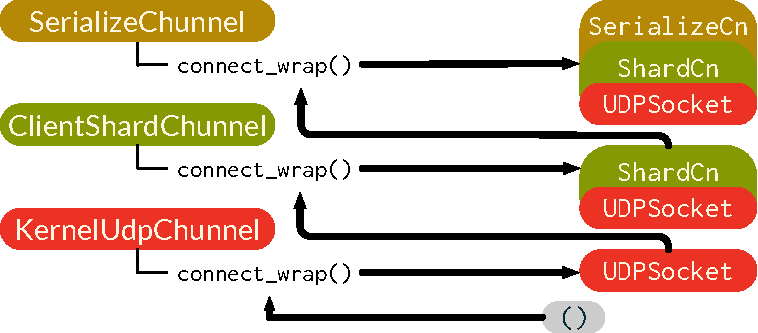
\includegraphics[width=\columnwidth]{img/chunnel-panda-proposal}
    \vspace{2pt}
    \caption{\name builds connections by recursively calling \tunnels' \texttt{connect\_wrap} functions. We show reconfiguration in \S\ref{s:reconfig}.}
    \label{f:chunnel}
\end{figure}

\subsection{The \tunnel Abstraction}\label{s:chunnel}
\tunnels are \name's core abstraction: each \tunnel represents a single communication function, \ie logic that can:
\begin{inparaenum}[(a)]
\item Transform data (\eg serializing, encrypting, or compressing data);
\item Decide where to send data (\eg which shard or DHT node should receive a request), or replicate data to multiple endpoints (\eg to implement publish-subscribe functionality); or
\item Send and receive data from hardware (\eg via DPDK or the OS networking stack)
\end{inparaenum}

Each \tunnel takes as input an existing connection $c$ and produces a new connection that encapsulates connection $c$ and adds the \tunnel's functionality to $c$.
Developers of communication libraries implement \tunnels to expose their library's functionality to application developers.
\tunnels are composable: composing two \tunnels creates a third \tunnel.\footnote{\tunnel composition is associative but not commutative.}
By composing \tunnels into \tunnel stacks, application developers can layer functionality into their connections: after applying one \tunnel to a connection, \name can apply another \tunnel to the resulting connection to create a connection that incorporates the features both \tunnels express.
To bootstrap a connection to start with, \tunnels that can appear at the bottom of the stack need to be able to transform a connection with no implementation (represented by a unit type in Rust).

We show an example of using a \tunnel stack in an application in Listing~\ref{l:chunnel-stack}.
Note that we implemented \name in Rust (we discuss this in \S\ref{s:impl}), and we thus describe our interfaces using Rust code. However, the core ideas and abstractions we describe here are general and are readily expressible in other languages.
On line $2$, we show an example of a \tunnel, the \texttt{KernelUdpChunnel}, that transforms the unit type into a UDP connection that can send and receive byte arrays.
On line $3$, we compose this with a \texttt{SerializeChunnel} that transforms this connection into one that exposes an object interface.
Then, on line $4$, we again compose this \tunnel with a sharding \tunnel. This produces a connection that can evaluate a sharding function and rewrite a message's destination address to the appropriate shard.
Finally, on line $5$ we make a \tunnel stack from these three \tunnels, and create a connection with all the specified features for the application.

\begin{listing}[t]
\begin{minted}[linenos, breaklines]{rust}
// A Chunnel control path.
pub struct AChunnel { /*...*/ }
// The ChunnelTransformer<R> trait implements connection establishment logic.
impl<R> ChunnelTransformer<R> for AChunnel
where R: ChunnelDatapath</*...*/>> {
  // Specify that AChunnelDP is the datapath used
  type Connection = AChunnelDP<R>;
  // Chunnel composition interface: compose AChunnel with inner.
  fn connect_wrap(&mut self, inner: R) -> 
    Self::Connection {/*...*/}
  // Specify relative compat. with other impls.
  type Capability = /*..*/;
  fn capabilities() -> Self::Capability { /*...*/ }
}
impl AChunnel {
  // Create a new AChunnel
  pub fn new(/*...*/) -> AChunnel { /* ... */}
}
// The AChunnel datapath
pub struct AChunnelDP<R>{/*...*/}
impl<R> ChunnelDatapath for AChunnelDP<R>
where R: /* input data type requirements */ {
  type Data = /*..*/;
  fn send(&self, ms: impl Iterator<Item=Self::Data>) { /*..*/ }
  fn recv(&self, buf: &mut [Option<Self::Data>]) { /*..*/ }
}
\end{minted}
\vspace{-11pt}
\caption{An overview of the \tunnel interface. Implementors of \texttt{ChunnelDatapath} are connection types, and implementors of \texttt{ChunnelTransformer} allow layering them.} \label{l:chunnel}
\vspace{-10pt}
\end{listing}

\subsection{Implementing a \tunnel}\label{s:chunnel-impl}
To expose their library's functionality as a \tunnel in \name, library developers provide a function that implements the transformer functionality as well as a returned connection type.
We show an example of how a library developer would implement these in Listing~\ref{l:chunnel}.
\name exposes the transformer functionality via the \texttt{ChunnelTransformer} trait (on line 4), and connection-level functionality via the \texttt{ChunnelDatapath} trait (on line 21).
The connection-level \texttt{ChunnelDatapath} trait is straightforward: it defines its data type (line 23) and functions to implement \texttt{send()} and \texttt{recv()}. \texttt{send()} accepts a batch of messages to send, and \texttt{recv()} waits for incoming messages and writes them into a caller-provided array. 

Meanwhile, the \texttt{ChunnelTransformer} trait's function, \texttt{connect\_wrap} (line 9) composes \tunnels in a connection. Figure~\ref{f:chunnel} shows this process. 
If \tunnel A appears above (\ie is pushed after) \tunnel B in a connection's stack, \name calls \tunnel A's \texttt{connect\_wrap} function with an \texttt{inner} argument corresponding to \tunnel B's \texttt{ChunnelDatapath} return type. 
\tunnel A's \texttt{connect\_wrap} function then returns a type that also implements \texttt{ChunnelDatapath}, \texttt{AChunnelDP}, whose data is first processed with \tunnel A's functionality and then passed to \tunnel B (by calling \texttt{ChunnelDatapath} methods on its inner \texttt{R}). 
Each \tunnel's \texttt{connect\_wrap} function is also responsible for performing connection initialization tasks, including initializing connection state, beginning connection handshake, etc. \name calls \texttt{connect\_wrap} recursively (starting with the bottom) on all \tunnels in the connection's stack, thus initializing all \tunnels used by the connection.

Observe that the \texttt{ChunnelTransformer} and \texttt{ChunnelDatapath} take the inner connection's type as a generic type parameter (\texttt{R}).
This allows the compiler to enumerate all possible connection types and optimize them at compile time, thus avoiding most dynamic dispatch overheads. %
We discuss how \name encapsulates reconfigurable \tunnels in \S\ref{s:impl}.

Developers can port existing libraries to \name by encapsulating their functionality in \tunnels.
We did this for our implementation, and as we discuss in \S\ref{s:impl}, the largest \tunnel we implemented is a DPDK \tunnel (1,700 lines of Rust code).
Most communication libraries are already designed to be composed with application logic and functionality from other libraries; \name's \tunnel abstraction merely enforces a unified interface that these libraries must implement. 
Indeed, \name does not require \tunnel implementations to be in Rust and implementations can use arbitrary third-party libraries. \tunnel developers must only specify the implementations their \tunnel is compatible with using \name's Rust interface.
This unified interface both simplifies composition and enables reconfiguration.
We have implemented several \tunnels and \name applications that we describe in \S\ref{s:applications}, demonstrating this abstraction's generality.

\paragrapha{\tunnel Datapath Type Safety}
\tunnel stacks are type-safe: in our implementation, we use the Rust type system\footnote{As we discuss in \S\ref{s:impl}, it is also possible to enforce this interface in languages other than Rust.} to ensure that when assembling a connection from a \tunnel stack, the data types of the resulting \texttt{ChunnelDatapath} will be compatible at each layer of encapsulation.
This is because \tunnel implementors specify their data type (\texttt{type Data} on line 23) as well as type restrictions on the connection type their \texttt{ChunnelTransformer} can accept (restrictions on \texttt{R} on line 5, restrictions elided).
\name imposes type restrictions on the input \tunnel stack (implemented as part of the \texttt{connect} function in Listing~\ref{l:chunnel-stack} line 5). So, if one of the \tunnels in a \tunnel stack does not match the others' data types, the application will fail to compile.
For example, a \tunnel that implements sharding needs access to a key that it can use to identify the correct shard. Such a tunnel can specify an input type such as \texttt{(String, Vec<u8>)} to indicate that it requires a string key to be passed along with the data. 
Naturally, datapath type safety does not extend across the network; this is why negotiation (\S\ref{s:negotiation}) is necessary.
